\documentclass[conference]{IEEEtran}
\IEEEoverridecommandlockouts
% The preceding line is only needed to identify funding in the first footnote. If that is unneeded, please comment it out.
\usepackage{cite}
\usepackage{amsmath,amssymb,amsfonts}
\usepackage{algorithmic}
\usepackage{graphicx}
\usepackage{textcomp}
\usepackage{xcolor}
\usepackage{listings}
\usepackage{hyperref}
\usepackage{xparse}


\definecolor{mGreen}{rgb}{0,0.6,0}
\definecolor{mGray}{rgb}{0.5,0.5,0.5}
\definecolor{mPurple}{rgb}{0.58,0,0.82}
\definecolor{backgroundColour}{rgb}{0.95,0.95,0.92}

\NewDocumentCommand{\codeword}{v}{%
	\texttt{\textcolor{blue}{#1}}%
}

\lstdefinestyle{CStyle}{
	backgroundcolor=\color{backgroundColour},   
	commentstyle=\color{mGreen},
	keywordstyle=\color{magenta},
	numberstyle=\tiny\color{mGray},
	stringstyle=\color{mPurple},
	basicstyle=\footnotesize,
	breakatwhitespace=false,         
	breaklines=true,                 
	captionpos=b,                    
	keepspaces=true,                 
	numbers=left,                    
	numbersep=5pt,                  
	showspaces=false,                
	showstringspaces=false,
	showtabs=false,                  
	tabsize=2,
	language=C
}

\lstset{language=C,keywordstyle={\bfseries \color{blue}}}

\def\BibTeX{{\rm B\kern-.05em{\sc i\kern-.025em b}\kern-.08em
    T\kern-.1667em\lower.7ex\hbox{E}\kern-.125emX}}
\begin{document}

\title{Weather Clock\\
{\footnotesize \textsuperscript{*}Echtzeit Datendarstellung auf dem Display}
}

\author{\IEEEauthorblockN{1\textsuperscript{st} Imron Gamidli}
\IEEEauthorblockA{\textit{Internationale Ingenieurwissenschaften} \\
\textit{Hochschule Fulda}\\
Fulda, Deutschland \\
imron.gamidli@lt.hs-fulda.de}
\and
\IEEEauthorblockN{2\textsuperscript{nd} Hussain Ali}
\IEEEauthorblockA{\textit{Internationale Ingenieurwissenschaften} \\
	\textit{Hochschule Fulda}\\
	Fulda, Deutschland \\
	husain.ali@lt.hs-fulda.de}
}

\maketitle

\begin{abstract}

\end{abstract}

\begin{IEEEkeywords}
dht22, arduino, uno, 
\end{IEEEkeywords}

\section{Einführung}
Dieses Projekt geht um ein Weather-Clock, dass es verschiedene Funktionen haben. Die Idee ist, eine Wetteruhr mit mehreren Funktionen zu haben, die verschiedene Merkmale von Wetter und Zeit messen und anzeigen kann. Die Funktionen werden flexibel und Portal sein. Man konnte die Funktion der Uhrzeit und des Datums ändern und auch die Eigenschaften des Wetters sehen. Die Motivation hinter diesem Projekt ist die Einsparung von Strom sowie die Berücksichtigung des Bildschirms durch einen Bewegungssensor, der neben seinen Funktionalitäten eine gute Initiative zum Energiesparen sein kann.


Wir haben viel über die Wetteruhr recherchiert, aber diese Energiesparfunktion hat gefehlt. Wir dachten, es wäre eine gute Idee, es zu haben. Wenn man sich im Raum oder in der Nähe des Bildschirms nicht befindet, sollte die Uhr oder das Display nicht eingeschaltet sein, wenn sich im Raum etwas bewegt, wird es wieder angezeigt. In der Zukunft kann man die Merkmale und Funktionen dieser Uhr erweitern und aktualisieren. Dies kann auch als Wecker verwendet werden. Da wir einen Bewegungssensor verwenden, um die Bewegung 
und das Drehen der Displayhelligkeit zu erfassen, kann man ihn auch als Alarm verwenden, um zu benachrichtigen, dass jemand kommt oder geht, insbesondere in öffentlichen Geschäften.

Es misst und zeigt die Uhrzeit, die Temperatur, die F¬euchtigkeit, den Luftdruck und die Höhenlage. Die Funktionen der Uhrzeit sind interaktiv, das heißt, kann man durch drei Knöpfen das Datum und Uhr andern und speichern. Die Darstellung von Uhr und Temperatur werden auf den zwei Displays gezeigt. Die beide sind 2x16 I2C Displays. 
Wir haben drei Sensoren, BMP280, DHT22, PIR verwendend. Der BMP280 misst der Luftdruck und die Höhenlage, der DHT22 misst die Temperatur, die Feuchtigkeit. Durch PIR Bewegung Sensor wird überprüft, wenn keine Bewegung in dem Raum ist, wird dann die Helligkeit von Displays ausgeschalten.

Außerdem wird RTC (Real Time Clock) benutzt, können wir dadurch die Echtzeit Uhr und Datum auf dem Display zeigen. Zudem RTC gibt es drei Knöpfen, die Funktionen von RTC andern und speichern lassen.  

Zum Protokoll verwenden wir I2C, mit dem kann man mehrere Slaves mit einem einzigen Master (wie SPI) verbinden und auch kann man mehrere Master haben, die einzelne oder mehrere Slaves steuern. Es ist sehr nützlich, wenn man mehr als ein Mikrocontroller Daten auf einer einzigen Speicherkarte protokolliert oder Text auf einem einzigen LCD anzeigt.


\section{DHT22 Sensor}

\subsection{Beschreibung}
Der DHT22 ist ein einfacher, preiswerter digitaler Temperatur- und Feuchtigkeitssensor. Er verwendet einen kapazitiven Feuchtigkeitssensor und einen Thermistor, um die Umgebungsluft zu messen, und spuckt ein digitales Signal auf dem Datenpin aus (keine analogen Eingangspins erforderlich). Er ist recht einfach zu bedienen, erfordert aber ein sorgfältiges Timing bei der Datenerfassung. Der einzige wirkliche Nachteil dieses Sensors ist, dass man nur alle 2 Sekunden neue Daten von ihm erhalten kann, so dass bei Verwendung unserer Bibliothek die Sensormesswerte bis zu 2 Sekunden alt sein können.

Verbinden Sie einfach den ersten Pin auf der linken Seite mit 3-5V Strom, den zweiten Pin mit Ihrem Dateneingangspin und den ganz rechten Pin mit Masse. Obwohl der Sensor ein einziges Kabel zum Senden von Daten verwendet, ist er nicht mit Dallas One Wire kompatibel! Wenn Sie mehrere Sensoren wünschen, muss jeder seinen eigenen Datenpin haben.

Im Vergleich zum DHT11 ist dieser Sensor präziser, genauer und funktioniert in einem größeren Temperatur-/Feuchtigkeitsbereich, ist aber auch größer und teurer.

Wird mit einem 4.7K - 10K Widerstand geliefert, den Sie als Pullup vom Daten-Pin zu VCC verwenden wollen.

\subsection{Technische Daten}
\begin{itemize}
	\item Geringe Kosten
	\item 3 bis 5V Stromversorgung und E/A
	\item Maximal 2,5 mA Stromverbrauch während der Umwandlung (während der Datenabfrage)
	\item Gut geeignet für 0-100% Luftfeuchtigkeit mit 2-5% Genauigkeit
	\item Gut geeignet für Temperaturmessungen von -40 bis 80°C mit einer Genauigkeit von ±0,5°C
	\item Abtastrate nicht mehr als 0,5 Hz (einmal alle 2 Sekunden)
	\item Gehäusegröße 27mm x 59mm x 13,5mm (1,05" x 2,32" x 0,53")
	\item 4 Stifte, 0,1" Abstand 
	\item Gewicht (nur der DHT22): 2,4g
\end{itemize}

	
\begin{figure}
	\begin{center}
		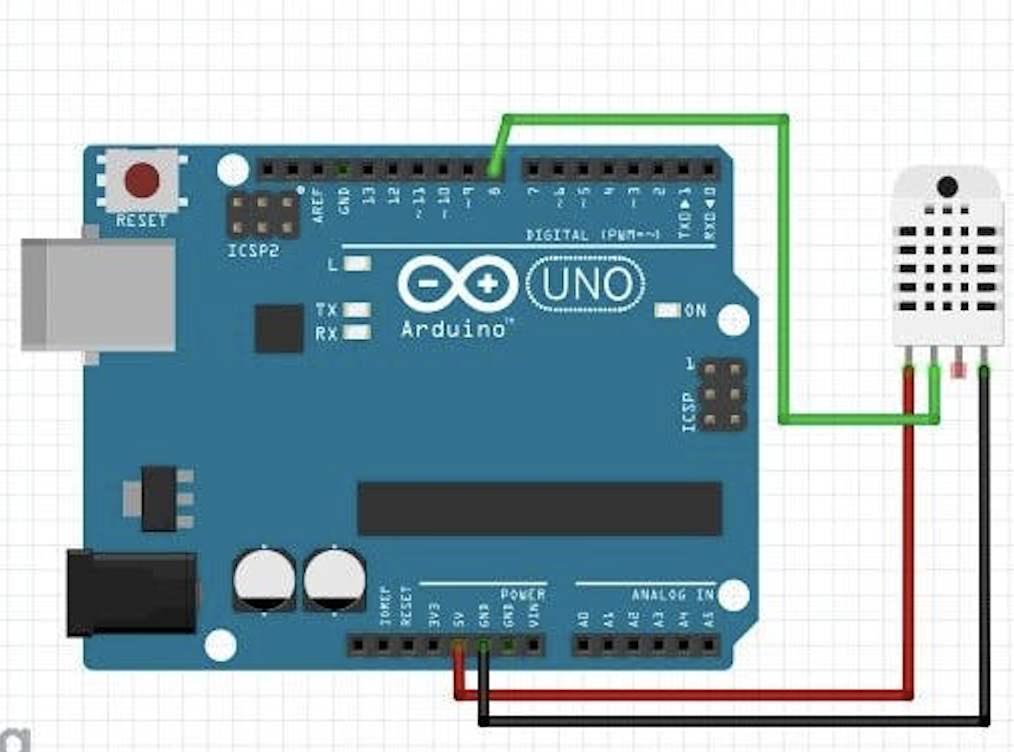
\includegraphics[scale=0.3]{dht22}
	\end{center}
	\caption{DHT22 Sensor}
\end{figure}

Es ist ziemlich einfach, die DHT-Sensoren anzuschließen. Sie haben vier Stifte VCC - roter Draht Schließen Sie an 3,3 - 5V Strom an. Manchmal reicht die 3,3-V-Spannung nicht aus, in diesem Fall versuchen Sie es mit einer 5-V-Spannung. Datenausgang - weißes oder gelbes Kabel Nicht angeschlossen Masse - schwarzes Kabel Ignorieren Sie einfach Pin 3, er wird nicht verwendet. Dieses Diagramm zeigt, wie wir für die Testskizze anschließen werden. Schließen Sie Daten an Pin 2 an, Sie können dies später auf jeden beliebigen Pin ändern.

\subsection{Implementierung im Projekt}
DHT22 war nützlich für unseres Projekt. Mithilfe diesen Sensor, bekommen wir Temperatur und Feuchtigkeit Daten. Damit es möglich wird, Sensordaten zu lesen, bestimmte Bibliothek muss installiert und importiert soll. Die Bibliothek für DHT22 heißt \textit{DHT sensor library} und installiert wurde vom \url{https://github.com/adafruit/DHT-sensor-library} . Nachdem wir die Bibliothek installiert haben, haben wir diese importiert.


\begin{lstlisting}[style=CStyle]
#include <DHT.h>;
\end{lstlisting}

Diese Bibliothek ermöglicht uns eine DHT Instanz initialisieren. Hier man sieht wir haben PIN 13 für DHT Kommunikation. Danach haben wir DHT22 Instanz erstellt.

\begin{lstlisting}[style=CStyle]
#define DHTPIN 13	// what pin we're connected to
#define DHTTYPE DHT22	// DHT 22 
DHT dht(DHTPIN, DHTTYPE);	// Initialize DHT 
\end{lstlisting}

Wir werden später Daten aus dem Sensor in Variablen speichern. Dafür haben wir zwei Variablen, \textsf{hum} für Feuchtigkeit und \textsf{temp} für Temperatur deklariert. 

\begin{lstlisting}[style=CStyle]
float hum;	//Stores humidity value
float temp;	//Stores temperature value
\end{lstlisting}

In \textsf{setup()} Funktion haben wir die DHT Instanz gestartet. Das heißt, die Instanz läuft und wir können jederzeit Feuchtigkeit und Temperaturdaten anfragen. 

\begin{lstlisting}[style=CStyle]
void setup()
{
	dht.begin();
}
\end{lstlisting}

In der Schleife \textsf{loop()} das Programm liest Feuchtigkeitswert mit \textsf{readHumidity()} und speichert in \textsf{hum} variable. Auf die gleiche Weise Temperatur wird mit \textsf{readTemperature()} gelesen und in \textsf{temp} gespeichert. 

\begin{lstlisting}[style=CStyle]
void loop()
{
	//Read data and store it to variables hum and temp
	hum = dht.readHumidity();
	temp = dht.readTemperature();
	
}
\end{lstlisting}

Letzte Aufgabe ist auf dem Display darzustellen, das vorher  mit entsprechender Adresse initialisiert wurde. Wir haben zwei Displays, für DHT Daten haben wir erste Reihe des erstens Display benutzt. 

\begin{lstlisting}[style=CStyle]
	void loop()
	{
		//Read data and store it to variables hum and temp
		hum = dht.readHumidity();
		temp = dht.readTemperature();
		
		lcd1.setCursor(0, 0);
		lcd1.print("tmp:");
		lcd1.print(temp); 
		lcd1.setCursor(6, 0);
		lcd1.print((char)223);
		lcd1.print("C hum:");
		lcd1.print(hum);
		lcd1.setCursor(15, 0);
		lcd1.print("%");
		
	}
\end{lstlisting}

\section{PIR Motion Sensor}
\subsection{Überblick}
PIR-Sensoren ermöglichen die Erfassung von Bewegungen und werden fast immer verwendet, um festzustellen, ob sich ein Mensch in den Sensorbereich hinein- oder herausbewegt hat. Sie sind klein, preiswert, stromsparend, einfach zu bedienen und verschleißen nicht. Aus diesem Grund werden sie häufig in Geräten und Vorrichtungen in Haushalten und Unternehmen eingesetzt. 
	
\begin{figure}
	\begin{center}
		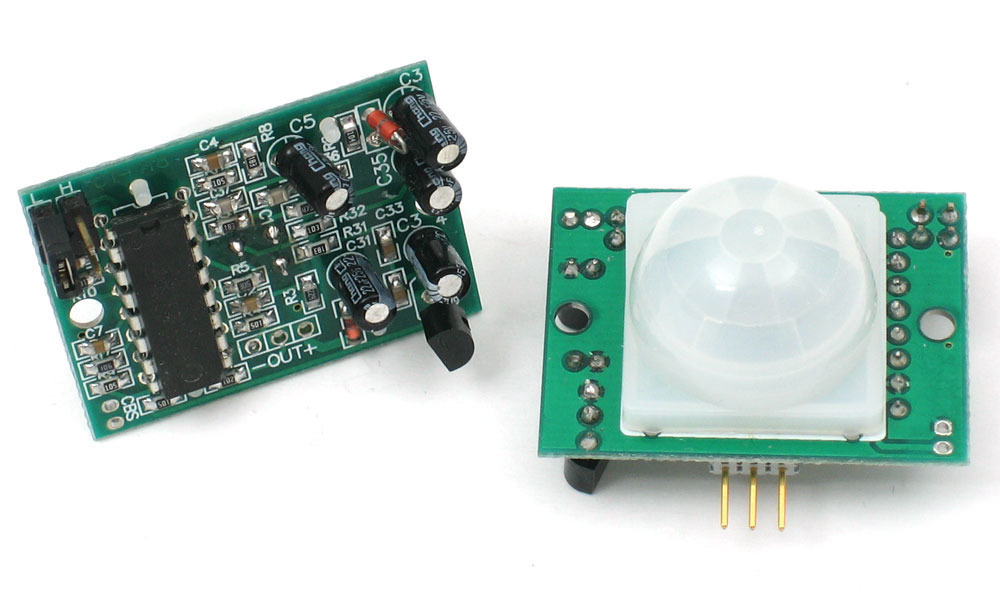
\includegraphics[scale=0.15]{pir1}
	\end{center}
	\caption{PIR Sensor}
\end{figure}

PIR-Sensoren bestehen im Wesentlichen aus einem pyroelektrischen Sensor (den Sie unten als runde Metalldose mit einem rechteckigen Kristall in der Mitte sehen können), der die Stärke der Infrarotstrahlung erkennen kann. Alles gibt eine schwache Strahlung ab, und je heißer etwas ist, desto mehr Strahlung wird freigesetzt. Der Sensor in einem Bewegungsmelder ist eigentlich in zwei Hälften geteilt. Der Grund dafür ist, dass wir eine Bewegung (Veränderung) und nicht die durchschnittliche IR-Stärke erkennen wollen. Die beiden Hälften sind so verdrahtet, dass sie sich gegenseitig aufheben. Wenn eine Hälfte mehr oder weniger IR-Strahlung sieht als die andere, schwankt der Ausgang nach oben oder unten.

\begin{figure}
	\begin{center}
		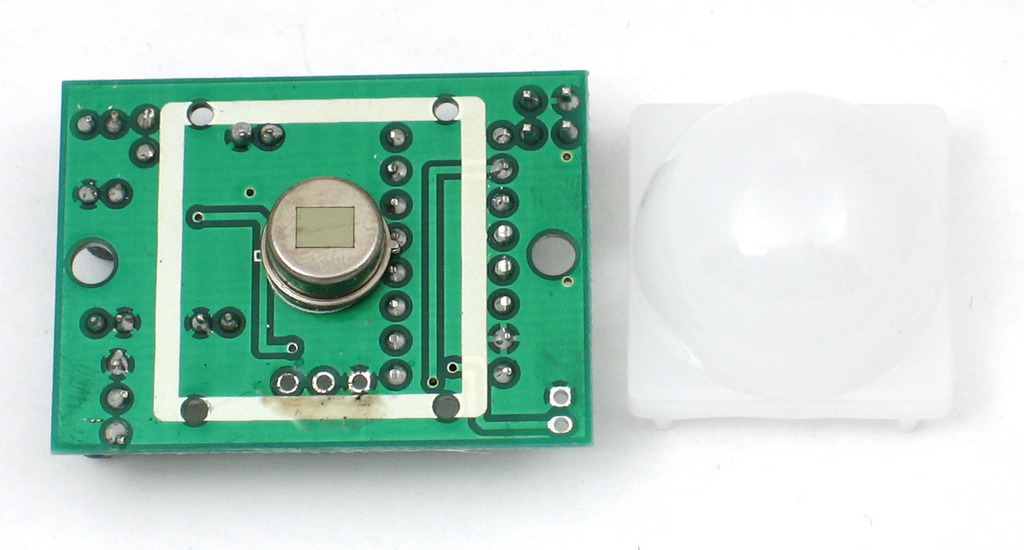
\includegraphics[scale=0.15]{pi2}
	\end{center}
	\caption{PIR Sensor 1}
\end{figure}

Zusammen mit dem pyroelektrischen Sensor gibt es eine Reihe von unterstützenden Schaltungen, Widerständen und Kondensatoren. Es scheint, dass die meisten kleinen Bastler-Sensoren den BISS0001 verwenden, zweifellos ein sehr preiswerter Chip. Dieser Chip nimmt das Ausgangssignal des Sensors auf und verarbeitet es ein wenig, um einen digitalen Ausgangsimpuls aus dem analogen Sensor zu erzeugen.

Im Vergleich zu älteren PIRs haben die neuen PIRs mehr einstellbare Einstellungen und sind mit einer Stiftleiste ausgestattet, die in den 3-poligen Masse-/Ausgangs-/Stromanschlüssen installiert ist.

\begin{figure}
	\begin{center}
		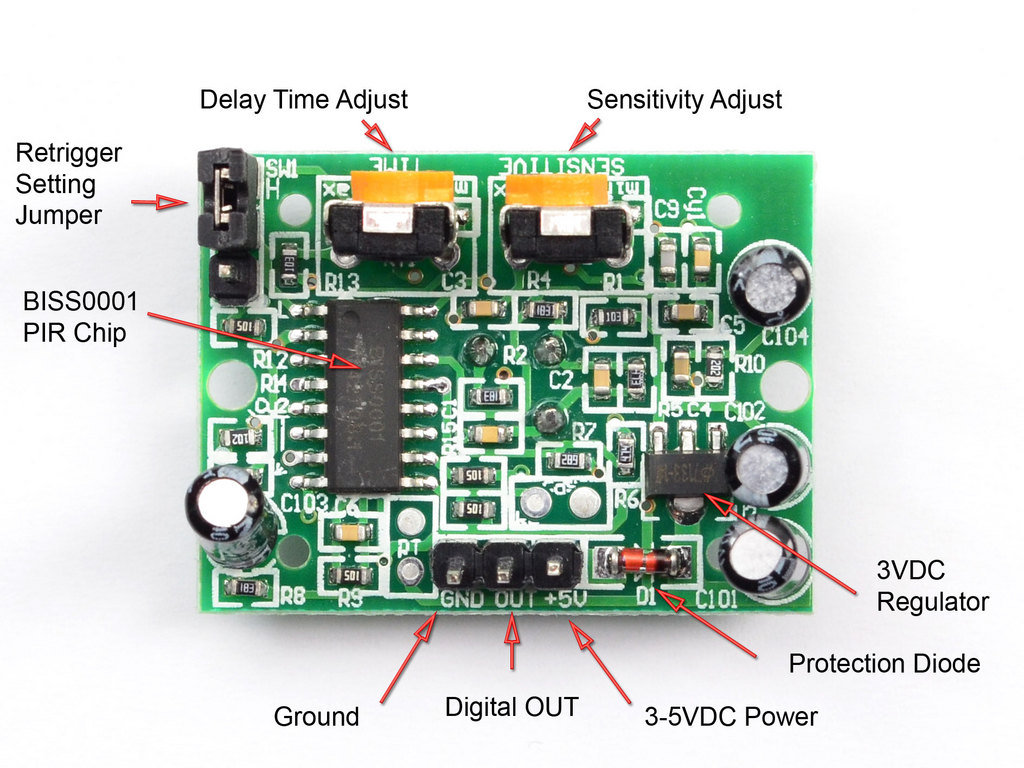
\includegraphics[scale=0.15]{pir3}
	\end{center}
	\caption{PIR Sensor Einstellungen}
\end{figure}

Für viele einfache Projekte oder Produkte, bei denen erkannt werden muss, ob eine Person den Bereich verlassen oder betreten hat oder sich ihm genähert hat, sind PIR-Sensoren hervorragend geeignet. Sie sind stromsparend und kostengünstig, ziemlich robust, haben einen großen Linsenbereich und sind einfach zu bedienen.  PIR-Sensoren zeigen nicht an, wie viele Personen sich in der Nähe aufhalten oder wie nah sie am Sensor sind. Die Linse ist oft auf einen bestimmten Bereich und eine bestimmte Entfernung festgelegt (obwohl sie irgendwo gehackt werden kann), und manchmal werden sie auch von Haustieren ausgelöst.

\subsection{Wie PIRs funktionieren}
PIR-Sensoren sind komplizierter als viele der anderen Sensoren, die in diesen Tutorials erklärt werden (wie Fotozellen, FSRs und Kippschalter), weil es mehrere Variablen gibt, die den Eingang und Ausgang des Sensors beeinflussen. Um zu erklären, wie ein grundlegender Sensor funktioniert, verwenden wir dieses schöne Diagramm

Der PIR-Sensor selbst hat zwei Schlitze. Jeder Schlitz besteht aus einem speziellen Material, das für IR empfindlich ist. Die Linse, die hier verwendet wird, macht nicht wirklich viel, und so sehen wir, dass die beiden Schlitze über eine gewisse Entfernung hinaus "sehen" können (im Grunde die Empfindlichkeit des Sensors). Wenn sich der Sensor im Leerlauf befindet, erkennen beide Schlitze die gleiche Menge an IR, nämlich die vom Raum, den Wänden oder der Außenumgebung abgestrahlte Menge. Wenn ein warmer Körper, z. B. ein Mensch oder ein Tier, vorbeikommt, fängt er zunächst eine Hälfte des PIR-Sensors ab, was eine positive Differenzänderung zwischen den beiden Hälften bewirkt. Wenn der warme Körper den Erfassungsbereich verlässt, geschieht das Gegenteil, wobei der Sensor eine negative Differenzänderung erzeugt. Diese Änderungsimpulse sind das, was erkannt wird.

\begin{figure}
	\begin{center}
		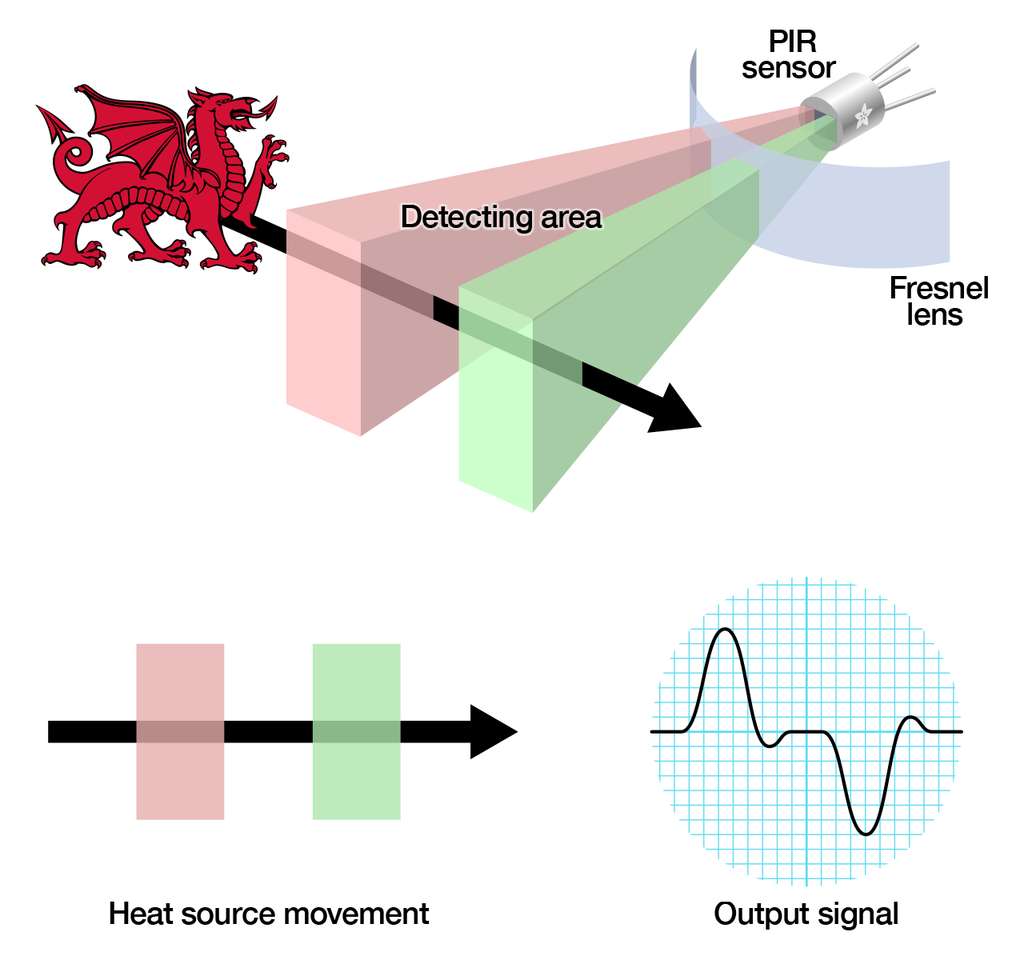
\includegraphics[scale=0.15]{pir4}
	\end{center}
	\caption{PIR Sensor Funktionsweise}
\end{figure}



\begin{figure}
	\begin{center}
		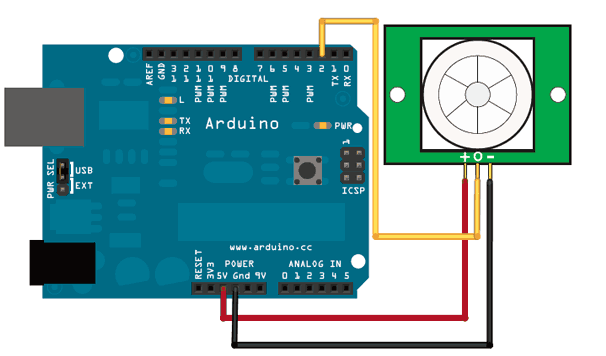
\includegraphics[scale=0.35]{pir5}
	\end{center}
	\caption{PIR Sensor Funktionsweise}
\end{figure}

\subsection{Implementierung im Projekt}
Wir haben Pin 2 im Arduino für PIR Sensor benutzt und starten wir das Programm mit keine Bewegung.  Für Lesen von PIN status, haben wir variable deklariert heißt val.

\begin{lstlisting}[style=CStyle]
int inputPin = 2;	// choose the input pin (for PIR sensor)
int pirState = LOW;	// we start, assuming no motion detected
int val = 0;	// variable for reading the pin status

\end{lstlisting}

Im Setup deklarieren wir inputPin (pin 2) als INPUT pin. Das ermöglicht Sensor zu lesen.

\begin{lstlisting}[style=CStyle]
void setup()
{
	pinMode(inputPin, INPUT);	// declare sensor as input
}
\end{lstlisting}\textbf{}

Im Loop passiert vieles. In jede Iteration wird  inputPin digital gelesen und  zum val gespeichert. Val kann jetzt HIGH oder LOW sein. Wenn val HIGH ist,  unsere Bildschirme werden beleuchtet.  Und wenn val LOW ist, das heißt es gibt keine Bewegung, dann werden Bildschirmlichten ausgeschaltet. 

\begin{lstlisting}[style=CStyle]
void loop()
{
	val = digitalRead(inputPin);	// read input value
	if (val == HIGH)
	{
		lcd.backlight();
		lcd1.backlight();
		if (pirState == LOW)
		{
			// we have just turned on
			Serial.println("Motion detected!");
			// We only want to print on the output change, not state
			pirState = HIGH;
		}
	}
	else
	{
		lcd.noBacklight();
		lcd1.noBacklight();
		if (pirState == HIGH)
		{
			// we have just turned of
			Serial.println("Motion ended!");
			// We only want to print on the output change, not state
			pirState = LOW;
		}
	}
}
\end{lstlisting}\textbf{}

\section{Real Time Clock }

\subsection{Überblick}

Dies ist eine großartige batteriegepufferte Echtzeituhr (RTC), die es Ihrem Mikrocontroller-Projekt ermöglicht, die Zeit zu verfolgen, selbst wenn es umprogrammiert wird oder die Stromversorgung ausfällt. Perfekt für die Datenerfassung, die Erstellung von Uhren, Zeitstempel, Timer und Alarme, usw. Der DS1307 ist der beliebteste RTC und funktioniert am besten mit 5V-basierten Chips wie dem Arduino.

\begin{figure}
	\begin{center}
		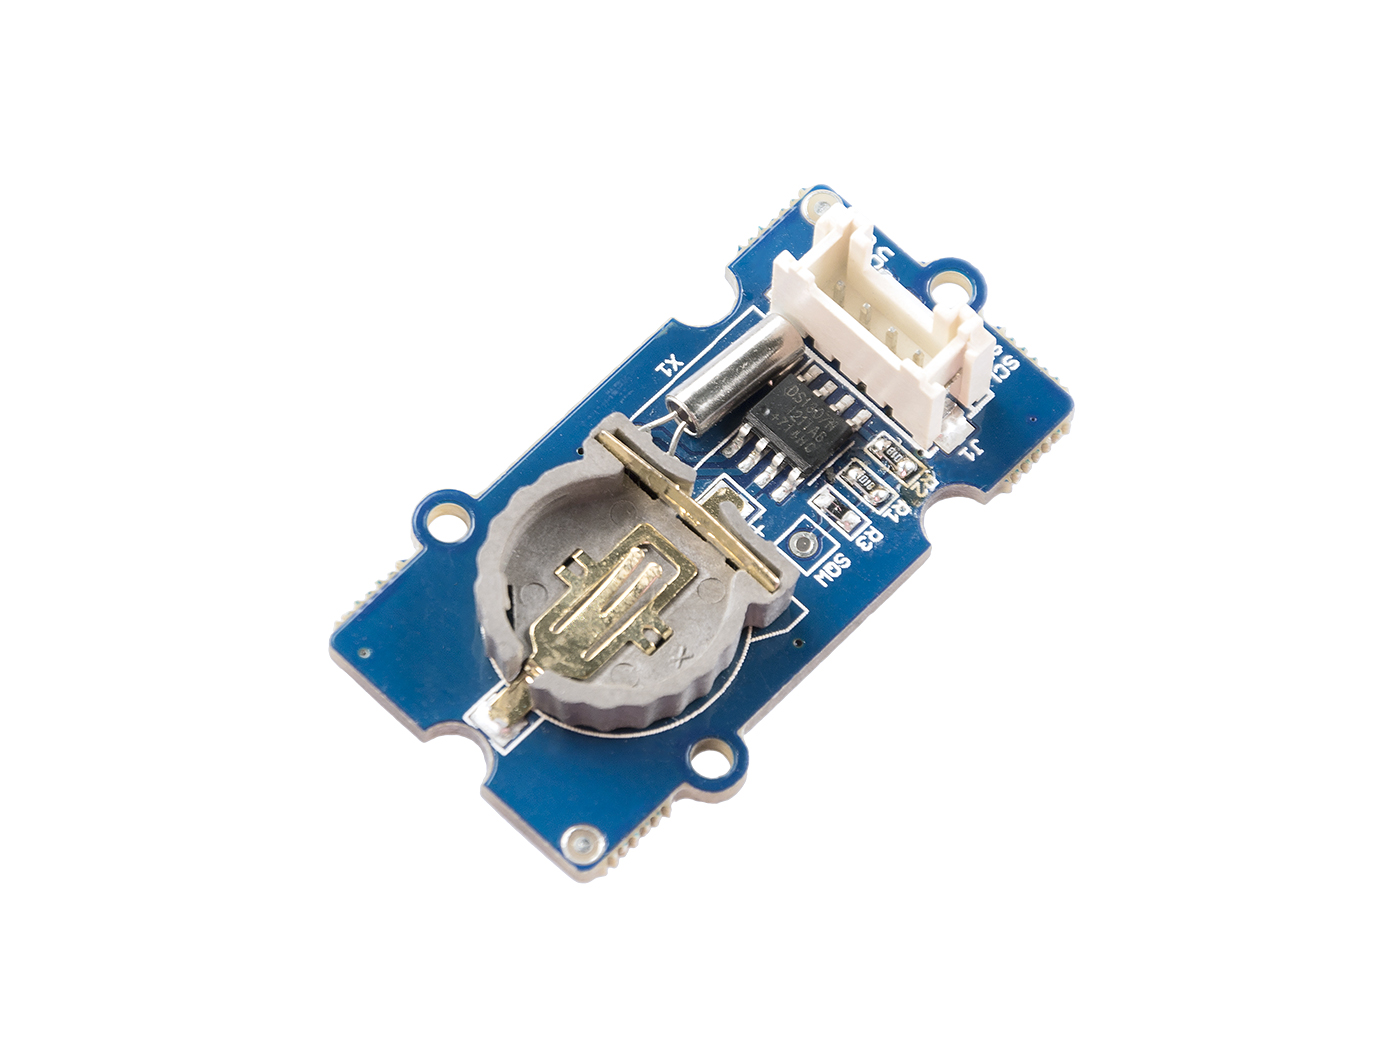
\includegraphics[scale=0.45]{rtc1}
	\end{center}
	\caption{RTC DS1307}
\end{figure}

\begin{itemize}
	\item Alle Teile, einschließlich PCB, Header und Batterie sind enthalten
	\item Schnell zu montieren und zu verwenden
	\item Kann in jedes Breadboard eingesteckt werden, oder Sie können Drähte verwenden
	\item Beispielcode und Bibliothek für Arduino mit einer Anleitung auf  Dokumentationsseite
	\item Zwei Befestigungslöcher
	\item Hält die Zeit für 5 Jahre oder länger
\end{itemize}


\subsection{Was ist ein RTC}
Eine Echtzeituhr ist im Grunde wie eine Uhr - sie läuft mit einer Batterie und behält die Zeit für Sie, auch wenn der Strom ausfällt! Mit einer RTC können Sie lange Zeiträume im Auge behalten, selbst wenn Sie Ihren Mikrocontroller neu programmieren oder ihn vom USB-Anschluss oder einer Steckdose abtrennen.

Die meisten Mikrocontroller, darunter auch der Arduino, haben einen eingebauten Zeitmesser namens millis(), und es gibt auch in den Chip eingebaute Timer, die längere Zeiträume wie Minuten oder Tage verfolgen können. Warum sollte man also einen separaten RTC-Chip haben wollen? Nun, der Hauptgrund ist, dass millis() nur die Zeit seit dem letzten Einschalten des Arduino erfasst. Das bedeutet, dass der Millisekunden-Timer auf 0 zurückgesetzt wird, wenn der Strom eingeschaltet wird. Der Arduino weiß nicht, dass es "Dienstag" oder "8. März" ist, er kann nur sagen: "Es sind 14.000 Millisekunden vergangen, seit ich das letzte Mal eingeschaltet wurde".

Was wäre, wenn Sie die Zeit auf dem Arduino einstellen wollten? Man müsste das Datum und die Uhrzeit einprogrammieren und könnte die Zeit von diesem Zeitpunkt an zählen lassen. Aber wenn der Strom ausfällt, muss man die Zeit neu einstellen. Ähnlich wie bei sehr billigen Weckern: Jedes Mal, wenn der Strom ausfällt, blinkt 12:00

Während diese Art der grundlegenden Zeitmessung für einige Projekte in Ordnung ist, benötigen einige Projekte wie Datenlogger, Uhren usw. eine konsistente Zeitmessung, die nicht zurückgesetzt wird, wenn die Arduino-Batterie stirbt oder umprogrammiert wird. Daher enthalten wir eine separate RTC! Der RTC-Chip ist ein spezieller Chip, der nur die Zeit misst. Er kann Schaltjahre zählen und weiß, wie viele Tage ein Monat hat, aber er kümmert sich nicht um die Sommerzeit (weil sie sich von Ort zu Ort ändert)

Die RTC, die wir verwenden werden, ist die DS1307. Sie ist preiswert, leicht zu löten und kann jahrelang mit einer sehr kleinen Knopfzelle betrieben werden.

Solange sie mit einer Knopfzelle betrieben wird, wird die RTC lange Zeit fröhlich vor sich hin ticken, auch wenn der Arduino die Stromversorgung verliert oder neu programmiert wird.

\begin{figure}
	\begin{center}
		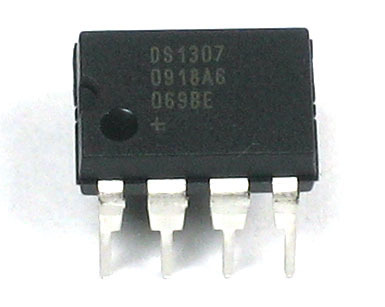
\includegraphics[scale=0.35]{rtc}
	\end{center}
	\caption{RTC DS1307}
\end{figure}

\subsection{Verdrahtung}

Es gibt nur 5 Pins: 5V GND SCL SDA SQW.

5V wird für die Stromversorgung des RTC-Chips verwendet, wenn Sie die Uhrzeit abfragen wollen. Wenn kein 5V-Signal anliegt, geht der Chip in den Ruhezustand und verwendet die Knopfzelle als Backup.
Verbinden Sie GND mit der gemeinsamen Strom-/Datenerde
Verbinden Sie den SCL-Pin mit dem SCL-Pin des I2C-Taktgebers an Ihrem Arduino. Bei einem UNO \& '328 basierten Arduino ist dies auch als A5 bekannt, bei einem Mega ist es auch als digital 21 bekannt und bei einem Leonardo/Micro, digital 3
Verbinden Sie den SDA-Pin mit dem I2C-Daten-SDA-Pin Ihres Arduino. Bei einem UNO- und '328-basierten Arduino ist dies auch als A4 bekannt, bei einem Mega ist es auch als digital 20 und bei einem Leonardo/Micro als digital 2 bekannt.
SQW ist der optional.

\subsection{Implementierung im Projekt}
Wir benutzen RTC, damit Arduino Zeit rechnet und auf dem Display anzeigt. Startet aber Uhr nicht richtig, dafür haben wir Buttons hinzufügt damit wir Uhrzeit korrekt einstellen können. Buttons diskutieren wir später. 

Für RTC braucht man zwei Bibliotheken: einmal DS1307 und ein mal RTClib.h. Hier haben wir diese Bibliotheken importiert. 

\begin{lstlisting}[style=CStyle]
#include "DS1307.h"
#include <RTClib.h>
\end{lstlisting}\textbf{}

Danach brauchen wir variable für DS1307 Objekt und für Uhrzeitkomponenten wir Stunde, Minute, Jahr, Monat und Tag. Hier sind die Variablen.

\begin{lstlisting}[style=CStyle]
DS1307 clock; //define a object of DS1307 class

int hourCnt;
int minagg;
int yearCnt;
int meseagg;
int dayagg;
\end{lstlisting}\textbf{}

Im Setup Funktion starten wir Uhr und setzen wir aktuellste Uhrzeit. Das ist Uhrzeit, in der wir dieses Projekt gemacht haben. Später kann man mit Buttons Uhrzeit ändern. 

\begin{lstlisting}[style=CStyle]
void setup(){
	//Clock
	clock.begin();
	clock.fillByYMD(2022, 1, 22); //Jan 19,2013
	clock.fillByHMS(20, 15, 0); //15:28 30"
	clock.fillDayOfWeek(SAT);//Saturday
	clock.setTime();//write time to the RTC chip
}
\end{lstlisting}\textbf{}

\subsection{Integration mit Buttons}
Push tasten oder Schalter verbinden zwei Punkte in einem Schaltkreis, wenn Sie sie drücken. In diesem Beispiel wird eine LED eingeschaltet, wenn die Taste einmal gedrückt wird, und ausgeschaltet, wenn sie zweimal gedrückt wird.

\begin{figure}
	\begin{center}
		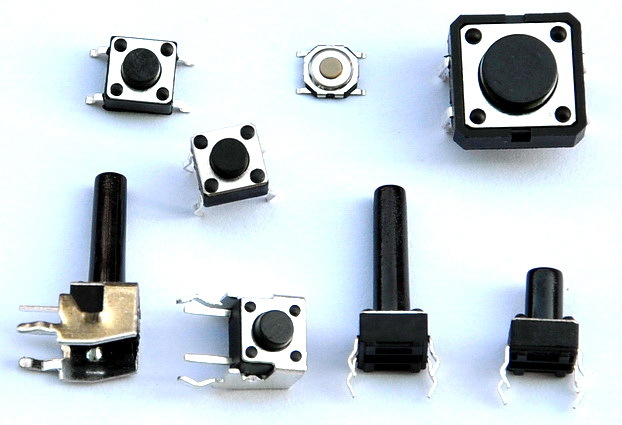
\includegraphics[scale=0.25]{btn}
	\end{center}
	\caption{Buttons}
\end{figure}

Wir haben drei Buttons benutzt und alle sind mit input pullup im Setup konfiguriert. 

\begin{lstlisting}[style=CStyle]
	void setup(){
		// Botton
		pinMode(P1,INPUT_PULLUP);
		pinMode(P2,INPUT_PULLUP);
		pinMode(P3,INPUT_PULLUP);
		int menu=0;
	}
\end{lstlisting}\textbf{}

Eine Taste ist für menu und es gibt insgesamt 6 Menus. Jede ist für set Stunde, Minute, Jahr, Monat,  Tag und letzte ist für Speicherung.  Hier sieht man, Button 1 input wird durch digitalRead(P1) gelesen und dann Menu entsprechend Funktion ausgeführt. 

\begin{lstlisting}[style=CStyle]
void loop(){
	 if(digitalRead(P1) == LOW)
	{
		menu=menu+1;
	}
	
	if (menu==0)
	{
		DisplayDateTime();
		
	}
	if (menu==1)
	{
		DisplaySetHour();
		
	}
	if (menu==2)
	{
		DisplaySetMinute();
	}
	if (menu==3)
	{
		DisplaySetYear();
		
	}
	if (menu==4)
	{
		DisplaySetMonth();
		
	}
	if (menu==5)
	{
		DisplaySetDay();
		
	}
	if (menu==6)
	{
		StoreAgg(); 
		delay(500);
		menu=0;
	}
	delay(100);
	}

}
\end{lstlisting}\textbf{}

\section{I2C LCD Display}
\subsection{Warum benutzen wir I2C}
Wenn Sie jemals versucht haben, ein LCD-Display mit einem Arduino zu verbinden, haben Sie vielleicht bemerkt, dass es eine Menge Pins am Arduino verbraucht. Selbst im 4-Bit-Modus benötigt der Arduino immer noch insgesamt sieben Anschlüsse - das ist die Hälfte der verfügbaren digitalen E/A-Pins des Arduino.

Die Lösung ist die Verwendung eines I2C-LCD-Displays. Es benötigt nur zwei I/O-Pins, die nicht einmal Teil eines Satzes digitaler I/O-Pins sind, und kann auch mit anderen I2C-Geräten gemeinsam genutzt werden.

\subsection{I2C LCD Hardware Übersicht}

Ein typisches I2C-LCD-Display besteht aus einem HD44780-basierten Zeichen-LCD-Display und einem I2C-LCD-Adapter. Lernen wir sie nacheinander kennen.

\subsubsection{Character LCD Display}
Wie ihr Name schon sagt, sind diese LCDs ideal für die Anzeige von Text/Zeichen. Ein 16×2-Zeichen-LCD hat beispielsweise eine LED-Hintergrundbeleuchtung und kann 32 ASCII-Zeichen in zwei Reihen mit je 16 Zeichen anzeigen.

\begin{figure}
	\begin{center}
		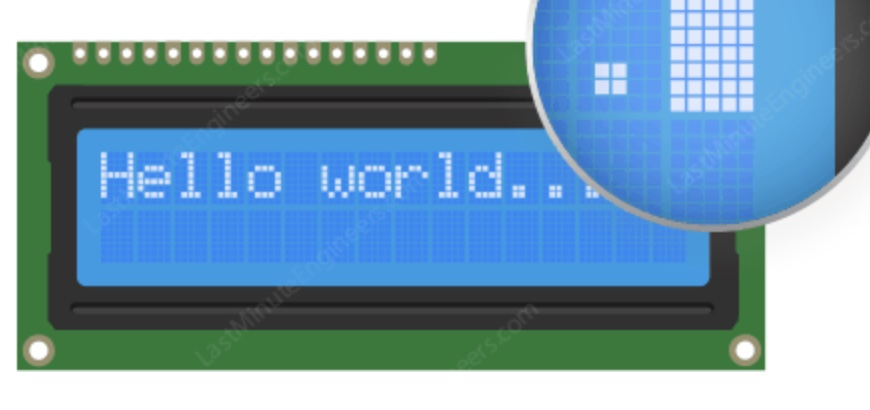
\includegraphics[scale=0.25]{dspl}
	\end{center}
	\caption{Pixeln in Display}
\end{figure}

Wenn Sie genau hinsehen, können Sie die kleinen Rechtecke für jedes Zeichen auf dem Display und die Pixel sehen, aus denen ein Zeichen besteht. Jedes dieser Rechtecke ist ein Raster von 5×8 Pixeln.

\subsubsection{I2C LCD Adapter}
Das Herzstück des Adapters ist ein 8-Bit I/O Expander Chip - PCF8574. Dieser Chip wandelt die I2C-Daten von einem Arduino in die vom LCD-Display benötigten parallelen Daten um.

\begin{figure}
	\begin{center}
		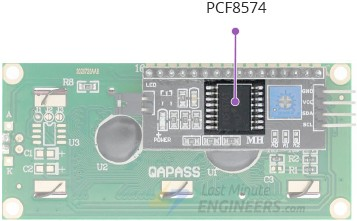
\includegraphics[scale=0.35]{dspl1}
	\end{center}
	\caption{PCF8574}
\end{figure}

Die Platine ist außerdem mit einem kleinen Trimpot ausgestattet, mit dem der Kontrast des Displays fein eingestellt werden kann.

Darüber hinaus befindet sich auf der Platine ein Jumper, der die Hintergrundbeleuchtung mit Strom versorgt. Um die Intensität der Hintergrundbeleuchtung zu steuern, können Sie den Jumper entfernen und eine externe Spannung an den mit "LED" gekennzeichneten Stift der Stiftleiste anlegen.


\begin{figure}
	\begin{center}
		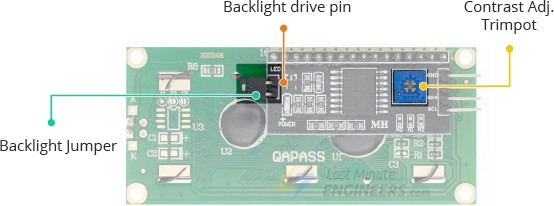
\includegraphics[scale=0.35]{dspl2}
	\end{center}
	\caption{Konfiguration von Display}
\end{figure}

\subsubsection{I2C Address of LCD}
Wenn Sie mehrere Geräte auf demselben I2C-Bus verwenden, müssen Sie möglicherweise eine andere I2C-Adresse für die Karte einstellen, damit sie nicht mit einem anderen I2C-Gerät in Konflikt gerät.

Dazu verfügt die Platine über drei Lötbrücken (A0, A1 und A2) oder Lötpads.

\begin{figure}
	\begin{center}
		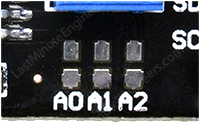
\includegraphics[scale=0.45]{dspl3}
	\end{center}
	\caption{Adresse setzen für Display}
\end{figure}

Jeder dieser Jumper wird zum Festcodieren der Adresse verwendet. Wenn ein Jumper mit einem Klecks Lötzinn kurzgeschlossen wird, wird die Adresse festgelegt.

Ein wichtiger Punkt dabei ist, dass viele Unternehmen den gleichen PCF8574-Chip herstellen: Texas Instruments und NXP Semiconductors, um nur einige zu nennen. Und die I2C-Adresse Ihres LCDs hängt vom Hersteller des Chips ab.


\subsubsection{Adresse finden im Projekt}
Wir haben zwei  Displays verwendet und die Adresse zu finden war kompliziert.  Wir haben einen kleinen Code geschrieben, damit wir die Adresse finden können. Hier ist der Code: 

\begin{lstlisting}[style=CStyle]
#include <Wire.h>
void setup() {
	Serial.begin (115200);
	while (!Serial)
	{
	}
	Serial.println ();
	Serial.println ("I2C scanner. Scanning ...");
	byte count = 0;
	Wire.begin();
	for (byte i = 8; i < 120; i++)
	{
		Wire.beginTransmission (i);
		if (Wire.endTransmission () == 0)
		{
			Serial.print ("Found address: ");
			Serial.print (i, DEC);
			Serial.print (" (0x");
			Serial.print (i, HEX);
			Serial.println (")");
			count++;
			delay (1); // maybe unneeded?
		} // end of good response
	} // end of for loop
	Serial.println ("Done.");
	Serial.print ("Found ");
	Serial.print (count, DEC);
	Serial.println (" device(s).");
} // end of setup
void loop() {}
\end{lstlisting}\textbf{}

\subsubsection{I2C LCD Display Pinout}

Ein I2C-LCD hat nur 4 Pins, die die Schnittstelle zur Außenwelt bilden. Die Anschlüsse sind wie folgt:
GND ist ein Masse-Pin und sollte mit der Masse des Arduino verbunden werden.

VCC versorgt das Modul und das LCD mit Strom. Schließen Sie ihn an den 5V-Ausgang des Arduino oder an eine separate Stromversorgung an.

SDA ist ein Pin für serielle Daten. Diese Leitung wird sowohl zum Senden als auch zum Empfangen verwendet. Schließen Sie ihn an den SDA-Pin des Arduino an.

SCL ist ein Pin für den seriellen Takt. Dies ist ein Taktsignal, das vom Bus-Master-Gerät geliefert wird. Schließen Sie es an den SCL-Pin des Arduino an.

\subsubsection{Verdrahtung}

Es ist viel einfacher, ein I2C-LCD anzuschließen als ein Standard-LCD. Sie müssen nur 4 Pins anstelle von 12 anschließen. Beginnen Sie mit dem Anschluss des VIN-Pins an den 5V-Ausgang des Arduino und verbinden Sie GND mit Masse.

Nun bleiben noch die Pins, die für die I2C-Kommunikation verwendet werden. Beachten Sie, dass jedes Arduino-Board unterschiedliche I2C-Pins hat, die entsprechend angeschlossen werden sollten. Bei den Arduino-Boards mit dem R3-Layout befinden sich SDA (Datenleitung) und SCL (Taktleitung) auf den Stiftleisten in der Nähe des AREF-Pins. Sie werden auch als A5 (SCL) und A4 (SDA) bezeichnet.

Nachdem Sie das LCD verdrahtet haben, müssen Sie den Kontrast des Displays einstellen. Auf dem I2C-Modul finden Sie ein Potentiometer, das Sie mit einem kleinen Schraubenzieher drehen können.

Stecken Sie den USB-Anschluss des Arduino ein, um das LCD mit Strom zu versorgen. Sie sollten sehen, dass die Hintergrundbeleuchtung aufleuchtet. Drehen Sie nun das Potentiometer, bis die erste Zeile des Rechtecks erscheint.

\subsubsection{Bibliothek}
Um die folgenden Sketche ausführen zu können, müssen Sie eine Bibliothek namens LiquidCrystal\_I2C installieren. Diese Bibliothek ist eine verbesserte Version der LiquidCrystal-Bibliothek, die mit Ihrer Arduino-IDE mitgeliefert wird.

Um die Bibliothek zu installieren, navigieren Sie zu Sketch > Include Library > Manage Libraries... Warten Sie, bis der Library Manager den Bibliotheksindex heruntergeladen und die Liste der installierten Bibliotheken aktualisiert hat.

Filtern Sie Ihre Suche durch Eingabe von 'liquidcrystal'. Es sollte ein paar Einträge geben. Suchen Sie nach LiquidCrystal I2C library von Frank de Brabander. Klicken Sie auf diesen Eintrag, und wählen Sie dann Installieren.

\subsection{Imlementierung im Projekt}

Der Sketch beginnt mit der Einbindung der LiquidCrystal\_I2C-Bibliothek.
\begin{lstlisting}[style=CStyle]
#include <LiquidCrystal_I2C.h>
\end{lstlisting}\textbf{}

Anschließend wird ein Objekt der Klasse LiquidCrystal\_I2C erstellt. Dieses Objekt verwendet 3 Parameter LiquidCrystal\_I2C(address,columns,rows). Hier müssen Sie die Standardadresse in die Adresse ändern, die Sie zuvor gefunden haben, falls sie anders ist, und die Abmessungen des Displays.

\begin{lstlisting}[style=CStyle]
LiquidCrystal_I2C lcd(0x3F,16,2);
\end{lstlisting}\textbf{}

Sobald das LiquidCrystal\_I2C-Objekt deklariert ist, können Sie auf spezielle Methoden zugreifen, die für das LCD spezifisch sind.

In der Funktion "setup" wird die Funktion init() aufgerufen, um das Objekt lcd zu initialisieren. Anschließend wird die Funktion clear() aufgerufen. Diese Funktion löscht den LCD-Bildschirm und verschiebt den Cursor in die obere linke Ecke. Mit der Funktion backlight() wird die Hintergrundbeleuchtung des LCD-Bildschirms eingeschaltet.

\begin{lstlisting}[style=CStyle]
lcd.init();
lcd.clear();         
lcd.backlight();
\end{lstlisting}\textbf{}

Als nächstes wird die Cursorposition auf die dritte Spalte und die erste Zeile des LCDs gesetzt, indem die Funktion lcd.setCursor(2,0) aufgerufen wird. Die Cursorposition gibt die Stelle an, an der der neue Text auf dem LCD angezeigt werden soll. Die linke obere Ecke wird als col=0, row=0 betrachtet.

\begin{lstlisting}[style=CStyle]
lcd.setCursor(2,0);
\end{lstlisting}\textbf{}

Anschließend wird die Zeichenkette "Hello World!" durch Aufruf der Funktion print() gedruckt.

\begin{lstlisting}[style=CStyle]
lcd.print("Hello world!");
\end{lstlisting}\textbf{}

In ähnlicher Weise setzen die nächsten beiden Zeilen den Cursor auf die dritte Spalte und die zweite Zeile und drucken 'LCD Tutorial' auf das LCD.

\begin{lstlisting}[style=CStyle]
lcd.setCursor(2,1);
lcd.print("LCD Tutorial");
\end{lstlisting}\textbf{}

Wir haben auch die Adressen gefunden und die Bibliothek eingebunden.
\begin{lstlisting}[style=CStyle]
#include <LiquidCrystal_I2C.h>

LiquidCrystal_I2C lcd(0x27, 16, 2); // I2C address 0x27, 16 column and 2 rows
LiquidCrystal_I2C lcd1(0x03F, 16, 2); // I2C address 0x03F, 16 column and 2 rows
\end{lstlisting}\textbf{}

Im Setup Funktion starten die beide Displays mit Rücklichter.

\begin{lstlisting}[style=CStyle]
lcd.init(); // initialize the lcd
lcd.backlight();

lcd1.init(); // initialize the lcd 1
lcd1.backlight();
\end{lstlisting}\textbf{}

Danach haben wir mit clear() und setCurson() Funktionen Informationen von Sensoren auf dem Display Dargestellt.



\begin{thebibliography}{00}
\bibitem{b1} https://github.com/adafruit/DHT-sensor-library
\bibitem{b2} https://github.com/semestrinis/Arduino/wiki/DHT22-temperature-humidity-sensor
\bibitem{b3} https://learn.adafruit.com/pir-passive-infrared-proximity-motion-sensor/overview
\bibitem{b4} https://learn.adafruit.com/pir-passive-infrared-proximity-motion-sensor/how-pirs-work
\bibitem{b5} https://learn.adafruit.com/pir-passive-infrared-proximity-motion-sensor/connecting-to-a-pir
\bibitem{b6} https://wiki.seeedstudio.com/Grove-RTC/
\bibitem{b7}
\end{thebibliography}
\vspace{12pt}


\end{document}
